\documentclass[tikz,border=10pt]{standalone}
\begin{document}
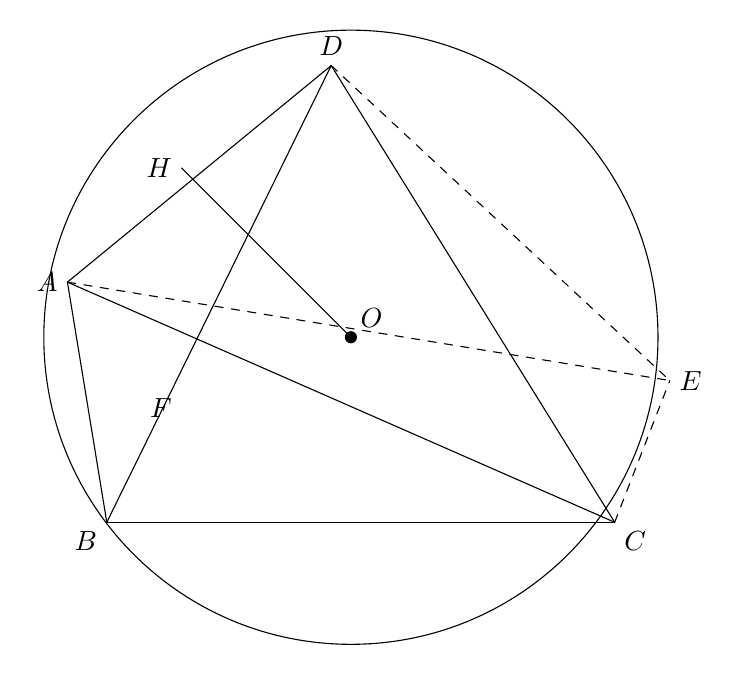
\begin{tikzpicture}[line cap=round,line join=round,scale=1]

% Circle center and radius
\coordinate (O) at (0,0);

% Points on the circle
\coordinate (A) at (-3.6,0.7);
\coordinate (B) at (-3.1,-2.35);
\coordinate (C) at (3.35,-2.35);
\coordinate (D) at (-0.25,3.45);
\coordinate (E) at (4.05,-0.55);

% Interior points
\coordinate (H) at (-2.15,2.15);
\coordinate (F) at (-2.15,-0.9);

% Outer circle
\draw (O) circle [radius=3.9];

% Solid chords/segments
\draw (A) -- (D);
\draw (A) -- (B);
\draw (A) -- (C);
\draw (B) -- (C);
\draw (B) -- (D);
\draw (D) -- (C);
\draw (H) -- (O);

% Dashed segments
\draw[dashed] (A) -- (E);
\draw[dashed] (D) -- (E);
\draw[dashed] (C) -- (E);

% Point O
\fill (O) circle (2.2pt);

% Labels
\node[left] at (A) {$A$};
\node[below left] at (B) {$B$};
\node[below right] at (C) {$C$};
\node[above] at (D) {$D$};
\node[right] at (E) {$E$};
\node[left] at (H) {$H$};
\node[left] at (F) {$F$};
\node[above right] at (O) {$O$};

\end{tikzpicture}
\end{document}
